\paragraph{Vertical Displacement $\delta$}

When an obstacle hexagon is rotated by $\alpha_i$, the height of the obstacle hexagon becomes $h \sec \alpha_i$ where $h$ is the canonical height of the obstacle hexagon (see Figure \ref{fig:hexagonNonCanonical.pdf} for reference).
Figure \ref{fig:hexagonNonCanonical.pdf} shows the geometry of a rotated obstacle hexagon.

\begin{minipage}{\linewidth}
\begin{center}
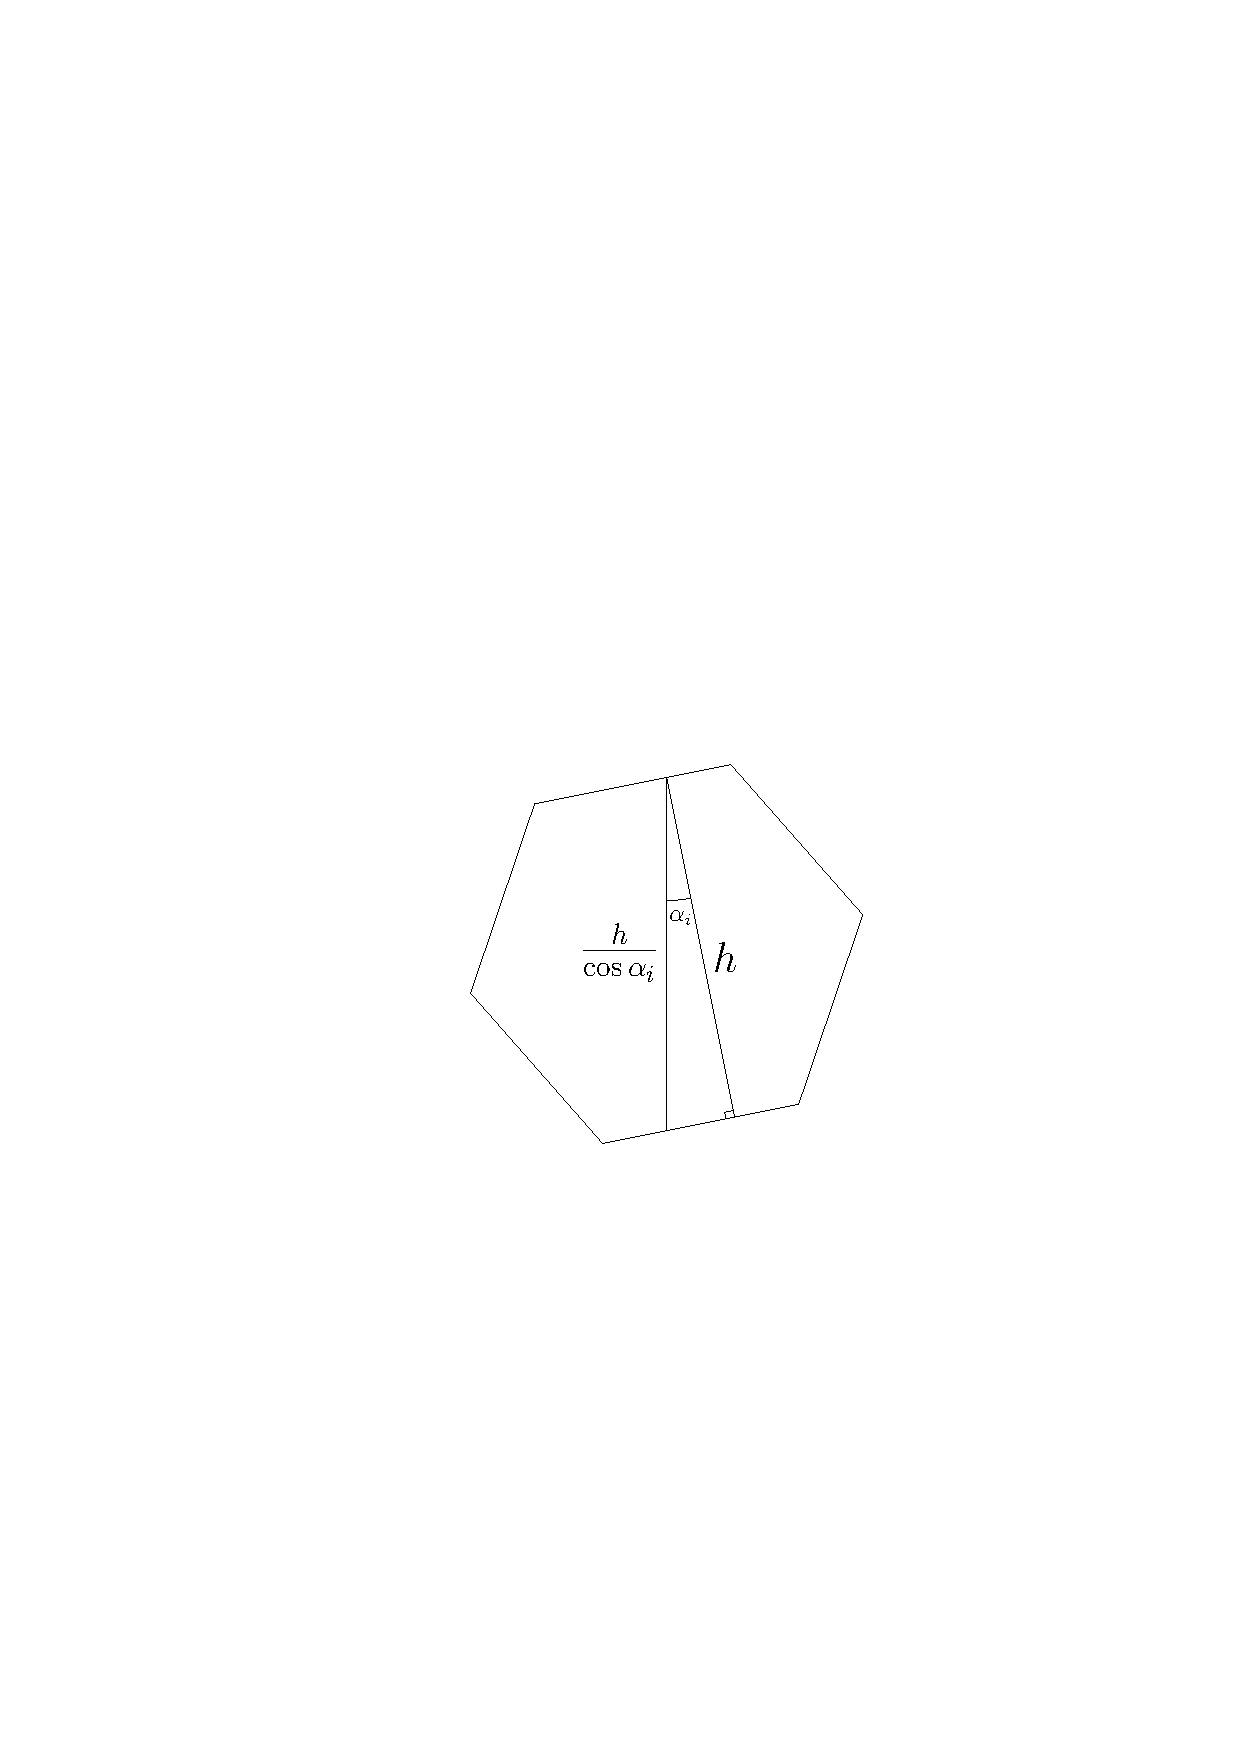
\includegraphics[width=.33\columnwidth]{graphics/hexagonNonCanonical2.pdf}
\captionof{figure}{
This figure shows a right triangle with angle $\alpha_i$ and sides of length $h$ and $\frac{h}{\cos \alpha_i}$.
}\label{fig:hexagonNonCanonical.pdf}
\end{center}
\end{minipage}

To show that the vertical displacement from canonical position is small, we first consider a column of obstacle hexagons in canonical position (see Figure \ref{fig:dualSmallHexagonalGrid.pdf} for illustration).  
For canonical position, the $\jth$ obstacle has $\delta_j = 0$.

\begin{minipage}{\linewidth}
\begin{center}
\includegraphics[width=.33\columnwidth]{graphics/verticalDisplacementArgument.pdf}
\captionof{figure}{This illustration is of a column of obstacle hexagons in canonical position along a vertical line segment $\ell$.}\label{fig:verticalDisplacementArgument.pdf}
\end{center}
\end{minipage}

From Equation \ref{eqn:Hnm}, we know the exact height of $\ell$ in terms of the heights of the corridors and obstacle hexagons in canonical position.  
Consider the first $j$ terms for the height of the column of obstacle hexagons and corridors for an arbitrary construction with angular rotation and vertical displacement for \textit{one} obstacle hexagon $\vert \delta_v \vert > 0$, where $j=2$, $\cdots$, $u+1$ and $1 < v \leq j$.
\begin{eqnarray*}
\sum_{i=1}^j \lr{2 \sqrt{3} N \sec \lr{ \alpha_i}} + \delta_v  + (j-1) \lr{\frac{1}{100N}+\sqrt{3}} &\leq& j \cdot 2 N \sqrt{3} + (j-1) \cdot \lr{\frac{1}{100N}+\sqrt{3}}\\
2 \sqrt{3} N \sum_{i=1}^j \sec \lr{\alpha_i} + \delta_ v &\leq& j \cdot 2 \sqrt{3} N \\
\sum_{i=1}^j \sec \lr{\alpha_i} + \delta_v &\leq& j\\
 \delta_v &\leq& j- \sum_{i=1}^j \sec \lr{\alpha_i}\\
 \delta_v &\leq& j - \lr{j - \sum_{i=1}^j \frac{\alpha_i^2}{2}}\\
\delta_v &\leq&  \sum_{i=1}^j \frac{\alpha_i^2}{2}
\end{eqnarray*}

Using Inequalities \ref{eqn:angularSumBound} and \ref{eqn:angularMaxBound}, we derive the following result:
$$
\begin{array}{rcl}
\sum_{i=1}^j \frac{\alpha_i^2}{2} &\leq& \frac{1}{2}\sum_{i=1}^j  \lr{ \frac{2}{s^\kappa} }^2\\
&\leq&\frac{1}{2}\cdot  \lr{\frac{2}{s^{\kappa}}}^2 \cdot j\\
&\leq&\frac{1}{2}\cdot  \lr{\frac{2}{s^{\kappa}}}^2 \cdot u\\
&\leq&\frac{48s}{2s^{2\kappa}}\\
&\leq&\frac{24}{s^{2\kappa-1}}\\  
\end{array}
$$

Thus we finally say that the bound for $\delta_v$, where $1<v\leq j\leq u$, is small:
\begin{equation}\label{eqn:verticalBound}
\delta_v \leq \frac{24}{s^{2\kappa-1}}
\end{equation}


\paragraph{\textit{A Refinement of the Angular Rotation Bound on $\alpha$}}
An obstacle hexagon can have at most a vertical displacement of $\delta_i$.  
A corridor's height can grow by $2 \delta_i$ should the obstacle below the corridor shift down by $-\delta_i$ and the obstacle above the corridor shift up $\delta_i$.  
We infer from our vertical bound Inequality \ref{eqn:verticalBound}:
$$\delta_i \leq \frac{12}{s^{2\kappa-1}}$$
By incorportating the new vertical bound, we extend the height of the corridor in Inequality \ref{eqn:alphaBound} to refine the bound on $\gamma_i$ and therefore $\alpha$ as such:
\begin{equation}\label{eqn:alphaBoundRefined}
\begin{array}{rcl}
\gamma_i & \leq & \tan^{-1} \lr{\frac{2 \delta_i}
									 {	\frac{5t -1}{4}	}
								}\\
&\leq& \frac{8 \frac{24}{s^{2\kappa-1}}	}
			  {	5s^\kappa -1}\\
&\leq& \frac{ 192 }
			  {	4s^\kappa	s^{2\kappa-1}} \\
&\leq& \frac{48}{s^{3\kappa-1}}\\
\end{array} 
\end{equation}

